\section{RunOff Application}
For the final sprint the focus was on getting the application to communicate with the matchmaking server to allow two users to connect and compete against each other. The goal was to create a prototype with the functionality most crucial to the projects original vision.

\subsection{User Interface} 
The user interface was re-designed such that when a user has selected a route to run they will be directed back to the matchmaking screen and a small toast is displayed informing the user of the name of the chosen route. The user can then press the "matchmake" button to start the matchmaking process while also navigating to the Run Progress activity. For a user to start a competitive run at this point the flow is as shown in \autoref{fig:userflow}

\begin{figure}[ht]
\begin{center}
 \caption{User Interface Flow}
 \label{fig:userflow}
 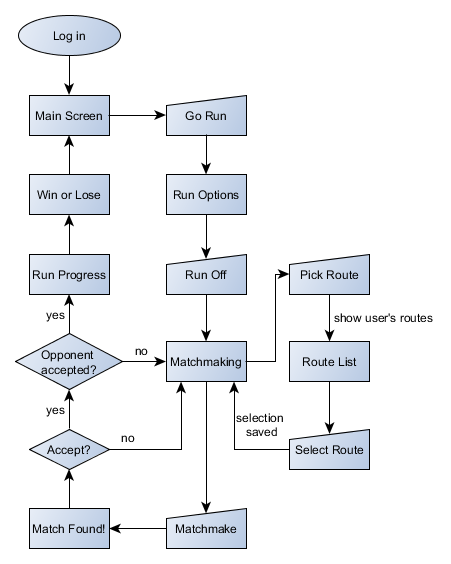
\includegraphics[scale=0.7]{img/runappflow.png}
\end{center}
\end{figure}

The main visual changes from the previous design of the Run Progress activity is a pop-up prompting the user to accept or decline a match as well as a toast counting down until the start of the race when both users have accepted. Once the race has started the Run Progress activity will start sending the position of the runner to the matchmaking server and listening for the position of the opponent. The progress of the opponent is shown relative to the user's own route such that if the opponent is 25\% done with their route, a marker will show up on the user's map indicating where the opponent would be on the user's route. The matchmaking server will at some point determine a winner and when the result is received a toast will be made indicating to the user if they are the winner or not.

The interface of the Run Progress activity should now look like \autoref{fig:mapMockV2}

\begin{figure}[ht]
\begin{center}
 \caption{Run Progress Mock-up}
 \label{fig:mapMockV2}
 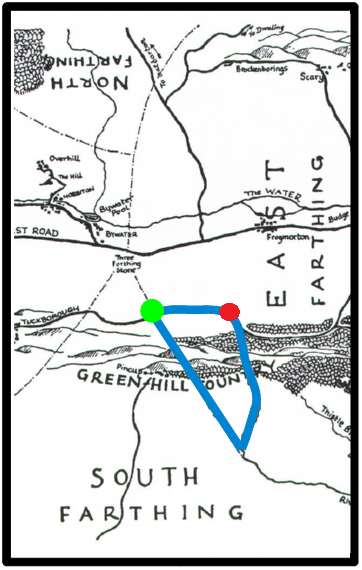
\includegraphics[scale=0.4]{img/mapMockV2.png}
\end{center}
\end{figure}

\subsection{Implementation}
The communication with the server was implemented with two new classes: \texttt{Message} and \texttt{Matchmaker} as well as an extension of the \texttt{RunProgress} activity and \texttt{GPSTracker} class. 
\vspace{10pt}

The \texttt{Message} class wraps the messages exchanged with the matchmaking server in a class with two constructors. There is one for outgoing messages, which simply sets local variables \texttt{cmd}, the type of command, \texttt{id}, the user-id and \texttt{data}, any needed data (can be null), to the given input parameters. These values can then be compiled into a \texttt{JSONObject} with the \texttt{compile()} method and encoded into a String for sending over a socket with the \texttt{get\_encoded()} method. 

The other constructor is for the received messages and it takes a \texttt{JSONObject} as its input parameter and sets the local variables to the values contained in the object.
\vspace{10pt}

The \texttt{Matchmaker} class handles the socket connection and the sending and receiving of messages from it. In the constructor of the class two \texttt{ConcurrentLinkedQueue}s are instantiated to handle the queueing of inbound and outbound messages. As well, it creates a new thread to handle the networking activity, seeing as Android does not allow these on the \ac{UI} thread. In the thread it creates a new socket and opens a connection to the \ac{IP} and port of the server. It also instantiates a \texttt{BufferedInputReader} to handle input (i.e. received messages) and a \texttt{DataOutputStream} for output for the socket. It starts a while loop, running while the socket is connected, which listens for incoming messages and sends outbound messages as long as the outbound queue is not empty.

Receiving new messages over a \ac{TCP} socket can be tricky as we can not ensure that the entire message is received in one piece or that we will only receive one message at a time. The message are therefore sent with two bytes in the front signifying how many characters are in the rest of the message.
\vspace{10pt}

As mentioned, the \texttt{RunProgress} activity has been extended as well. When the activity is first started it now creates a new instance of the \texttt{Matchmaker} class and sends a message to the server asking to be added to the queue of players waiting to be matched against an opponent. Once every second it checks the inbound queue for new messages and handles them according to which type is received:

\begin{itemize}
\item If the command is of the type FOUND a prompt is displayed to the user, asking them to either accept or decline the match. If they decline they are directed back to the \texttt{Matchmake} activity and from there they can choose to enqueue again. If they accept the match a message is sent to the server signalling this
\item When both parties have accepted the server sends its START message. When this message is received a countdown is started, counting down 10 seconds until the race starts.
\item Once the race is started the application starts receiving POSITION messages from the server. These contain information on how far along the opponent is along their route, sent as a fraction. This fraction is used to place the opponents marker on the map by using the checkpoints of the polyline. If an opponent is 20\% done with their route, the marker is placed at the checkpoint closest to 20\% done with the player's route. 
\item The final message is the WINNER message. This sends the winner's id. A toast is displayed informing the user of which player won the race.
\end{itemize}
\vspace{10pt}

For the \texttt{GPSTracker} service the only change is that the \texttt{onLocationChanged} function now sends a POSITION message to the server with the new coordinates.

\subsection{Testing}
As unit tests require predictable outcomes to pass they are not well suited for testing sockets. If sockets were to be unit tested it would require two computers to behave exactly the same each time the test was run and it would also require no hiccups in the connection. It is possible to create mock-connections but there was not time to add another framework to the project at this point. Thus no new unit tests were written for the \texttt{RunProgress} activity and no unit tests were written for the \texttt{Matchmaker} class. However unit tests were written for the \texttt{Message} class.
The code coverage at the end of the sprint can be seen in \autoref{tab:emma4}

\begin{figure}[ht]
\caption{EMMA coverage results}
\label{tab:emma4}
\begin{tabular}{| c | c | c | c | c |}
\hline
class & method & block & line & name \\ \hline
67\% (20/30) & 53\% (79/150) & 49\% (1122/2286) & 49\% (295/600) & all classes \\
\hline
\end{tabular}
\vspace{10pt}

\begin{tabular}{| l | l |}
\hline
OVERALL STATS SUMMARY: & \\ \hline
total packages: & 1 \\
total classes: & 3 \\
total methods: & 150 \\
total executable files: & 12 \\
total executable lines: & 600 \\
\hline
\end{tabular}
\end{figure}

The coverage at this point is somewhat low, however this is in part due to the fact that many methods are auto-generated and that there, as mentioned, are no unit tests for some classes.